\labelchapter{objects1}{Objects}

Object-oriented programming is a programming model based on ``objects'' and their interactions.  The
OCaml object system, like many other object-oriented languages, includes various concepts
like objects, classes, inheritance, subtype polymorphism, \emph{etc}.
OCaml's object system also differs from other languages in several ways.  It is quite expressive,
and it is \emph{structural} rather than \emph{nominal}, meaning that the names of objects and
classes make very little difference.  We'll point out some of these differences as we go along.  For
now, let's start with simple objects, without classes.  We'll look at classes and inheritance in
Chapter~\ref{chapter:classes}, and we'll cover polymorphic classes in
Chapter~\ref{chapter:polyclasses}.

\index{objects!fields} 
\index{objects!methods}
\index{object@\lstinline/object $\cdots$ end/}
%
To begin, it is simplest to think of an object as a collection of data together with functions to
operate on that data.  The data are called \emph{fields} of the object, and the functions are called
\emph{methods}.  For example, the following object represents a polygon that includes a method
\hbox{\lstinline/draw/} to draw it on the screen (this examples uses the OCaml
\hbox{\lstinline/Graphics/} package to perform the drawing).

\label{keyword:val(objects)}
\label{keyword:object}
\label{keyword:method}
\begin{ocaml}
# #load "graphics.cma";;  (* Load the Graphics module into the toploop *)
# let poly =
  object
     val vertices = [|(46, 70); (54, 70); (60, 150); (40, 150)|]
     method draw = Graphics.fill_poly vertices
  end;;
@
\begin{topoutput}
val poly : < draw : unit > = <obj>
\end{topoutput}
@
\end{ocaml}
%
The syntax for an object uses the keywords \hbox{\lstinline/object $\cdots$ end/} as delimiters.  
Fields are defined with the keyword \hbox{\lstinline/val/}, and methods are defined with the
keyword \hbox{\lstinline/method/}.

\label{object-types}
\index{object types}
\index{objects!type}
The type of an object is similar to a record type, but it uses angle brackets
%
\hbox{\lstinline/< $\cdots$ >/} as delimiters.
The object type includes the method types, but not the types of the fields, so the type of
the polygon is simply \hbox{\lstinline/< draw : unit >/}.  It is easy to define other objects with the same
type.

\begin{ocaml}
# let circle =
  object
     val center = (50, 50)
     val radius = 10
     method draw =
        let x, y = center in
        Graphics.fill_circle x y radius
  end;;
@
\begin{topoutput}
val circle : < draw : unit > = <obj>
\end{topoutput}
@
\end{ocaml}
%
\index{\#!method invocation}
\index{objects!method invocation}
Methods are invoked by with the syntax \hbox{\lstinline/$\nt{object}$#$\nt{method-name}$/} (this is
often called \emph{sending a message} to the object).  The following sequence of operations opens the
graphics window, draws the two objects, and waits for a button to be pressed.  The display is shown on the
right.

\begin{center}
\begin{tabular}{cc}
\begin{minipage}[b]{3.5in}
\begin{ocamllisting}
Graphics.open_graph " 200x200";;
poly#draw;;
circle#draw;;
ignore (Graphics.wait_next_event [Graphics.Button_down]);;
\end{ocamllisting}
\end{minipage}
&
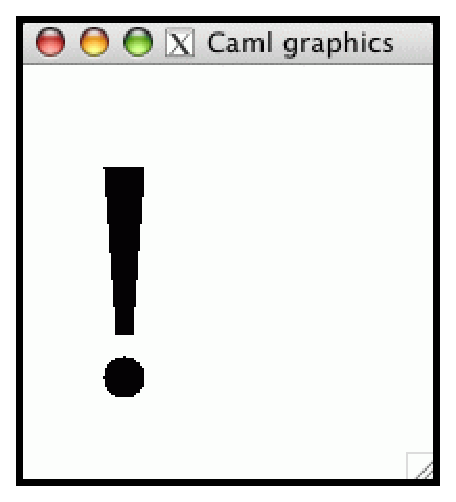
\includegraphics[scale=0.3]{graphics1}
\end{tabular}
\end{center}
%
\index{objects!dynamic lookup}
%
This example illustrates a property of object-oriented programming called \emph{dynamic lookup}.
%
\footnote{Dynamic lookup is often called \emph{polymorphism} in object-oriented circles, but that
  conflicts with the term \emph{polymorphism} that we use for ML.  The two are not at all the same.
  Following Mitchell~\cite{Mit03}, we'll use the term polymorphism to refer to \emph{parametric
    polymorphism} (type polymorphism), and \emph{dynamic lookup} to refer to object polymorphism.}
%
For an expression \hbox{\lstinline/obj#m/}, the actual method \hbox{\lstinline/m/} that gets called is determined
dynamically by the object \hbox{\lstinline/obj/}, not by some static property of the program.  A polygon
draws itself one way, a circle draws itself in another way, but the implementation is the
responsibility of the object, not the client.

\section{Encapsulation and polymorphism}
\label{section:object-constraint}
\index{row polymorphism}
\index{objects!encapsulation}

Another important feature of object-oriented programming is \emph{encapsulation}, also
called \emph{abstraction}.  An object encapsulates some data with methods for operating on the data;
it isn't necessary to know how an object is implemented in order to use it.  In our example, the
polygon and the circle have a single method \hbox{\lstinline/draw/}, so they have the same type, and they
can be used in the same ways.  Let's define a function to draw a list of objects.

\begin{ocaml}
# let draw_list items =
     List.iter (fun item -> item#draw) items;;
@
\begin{topoutput}
val draw_list : < draw : unit; .. > list -> unit = <fun>
\end{topoutput}
@
# draw_list [poly; circle];;
@
\begin{topoutput}
- : unit = ()
\end{topoutput}
@
\end{ocaml}
%
\index{row variables}
\index{row polymorphism}
\index{..@\lstinline/../ (in an object type)}
\label{keyword:..}
Note the type of the function \hbox{\lstinline/draw_list/}, which specifies that it takes a list of objects
of type \hbox{\lstinline/< draw : unit; .. >/}.  The ellipsis \hbox{\lstinline/../} in this type stands for ``other''
methods.  That is, the function \hbox{\lstinline/draw_list/} takes a list of objects having at least a
method \hbox{\lstinline/draw : unit/}, and possibly some other methods.  Suppose we defined a new kind of
object that represents a square that, in addition to having a method \hbox{\lstinline/draw/}, also defines
a method \hbox{\lstinline/area/} to compute the area.

\begin{center}
\begin{tabular}{cc}
\begin{minipage}[b]{3in}
\begin{ocamllistingx}
# let square =
  object
     val lower_left = (100, 100)
     val width = 10
     method area = width * width
     method draw =
        let (x, y) = lower_left in
        Graphics.fill_rect x y width width
  end;;
@
\begin{topoutput}
val square : < area : int; draw : unit > = <obj>
\end{topoutput}
@
# draw_list [square];;
@
\begin{topoutput}
- : unit = ()
\end{topoutput}
@
\end{ocamllistingx}
\end{minipage}
&
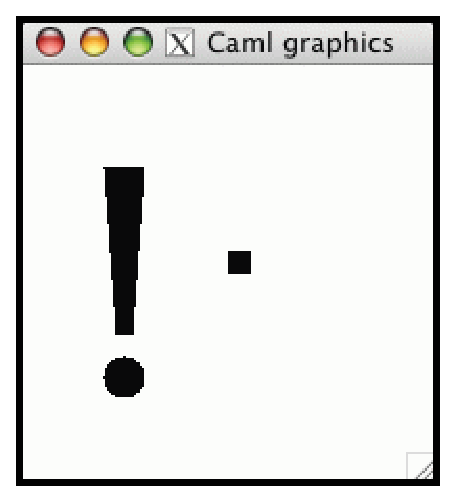
\includegraphics[scale=0.3]{graphics1a}
\end{tabular}
\end{center}
%
If we had used the simpler type \hbox{\lstinline/draw_list_exact : < draw : unit > list -> unit/}, the list
drawing function would work only with objects having \emph{exactly one} method, the
method \hbox{\lstinline/draw/}.  The expression \hbox{\lstinline/draw_list_exact [square]/} produces a type error,
because the object \hbox{\lstinline/square/} has an extra method \hbox{\lstinline/area/}.

\begin{ocaml}
# let draw_list_exact (items : < draw : unit > list) =
     List.iter (fun item -> item#draw) items;;
@
\begin{topoutput}
val draw_list_exact : < draw : unit > list -> unit = <fun>
\end{topoutput}
@
# draw_list_exact [square];;
@
\begin{toperror}
Characters 17-23:
  draw_list_exact [square];;
                   ^^^^^^
This expression has type < area : int; draw : unit >
but is here used with type < draw : unit >
The second object type has no method area
\end{toperror}
@
\end{ocaml}
%
Technically speaking, an occurrence of an ellipsis \hbox{\lstinline/../} in an object type is called a \emph{row
variable}, and the scheme for typing is called \emph{row polymorphism}.  It might not look like it,
but the type is really polymorphic, as we'll see if we try to write a type definition.

\begin{ocaml}
# type blob = < draw : unit; ..>;;
@
\begin{toperror}
Characters 4-30:
  type blob = < draw : unit; ..>;;
      ^^^^^^^^^^^^^^^^^^^^^^^^^^
A type variable is unbound in this type declaration.
In definition < draw : unit; .. > as 'a the variable 'a is unbound
\end{toperror}
@
\end{ocaml}
%
\label{keyword:as(object-types)}
\label{keyword:constraint}
\index{as!in object types}
\index{constraint@\lstinline/constraint/ (in object types)}
The issue is that an ellipsis \hbox{\lstinline/../} is like a type variable, standing for the types of all the
``other'' methods.  Unfortunately, it doesn't look like a type variable, and it doesn't make sense to
write \hbox{\lstinline/type (..) blob = < draw : unit; .. >/}.  The error message is a little cryptic, but
it suggests the solution, which is to introduce a type variable \hbox{\lstinline/'a/} that stands for the
type of the entire object.  The \hbox{\lstinline/as/} form and the \hbox{\lstinline/constraint/} form are
equivalent; you can write it either way.

\begin{ocaml}
# type 'a blob = < draw : unit; .. > as 'a;;
@
\begin{topoutput}
type 'a blob = 'a constraint 'a = < draw : unit; .. >
\end{topoutput}
@
# let draw_list_poly : 'a blob list -> unit = draw_list;;
@
\begin{topoutput}
val draw_list_poly : < draw : unit; .. > blob list -> unit = <fun>
\end{topoutput}
@
# draw_list_poly [square];;
@
\begin{topoutput}
- : unit = ()
\end{topoutput}
@
\end{ocaml}

\labelsection{objects-functional-update}{Transformations}

\index{transformation matrices}
%
An important feature of any 2D graphics library is the ability to transform objects by scaling,
rotation, or translation.  The cleanest way to do this is to make use of so-called \emph{homogeneous
  coordinates}, where the 2D coordinates $(x, y)$ are represented as triples $(x, y, 1)$, and
transformations are represented as $3{\times}3$ \emph{transformation matrices}.  A $3{\times}3$
matrix has 9 values $t_{ij}$, written as follows.

$$
\left(
\begin{array}{ccc}
t_{11} & t_{12} & t_{13}\\
t_{21} & t_{22} & t_{23}\\
t_{31} & t_{32} & t_{33}
\end{array}
\right)
$$
%
The product of a matrix and a vector is computed as follows, where $a b$ represents the product
of $a$ and $b$.

$$
\begin{array}{l}
\left(
\begin{array}{ccc}
t_{11} & t_{12} & t_{13}\\
t_{21} & t_{22} & t_{23}\\
t_{31} & t_{32} & t_{33}
\end{array}
\right)

\left(
\begin{array}{c}
x\\
y\\
z
\end{array}
\right)

=

\left(
\begin{array}{c}
t_{11} x + t_{12} y + t_{13} z\\
t_{21} x + t_{22} y + t_{23} z\\
t_{33} x + t_{23} y + t_{33} z
\end{array}
\right)
\end{array}
$$
%
The product of two matrices is computed as follows,

$$
\begin{array}{l}
\left(
\begin{array}{ccc}
s_{11} & s_{12} & s_{13}\\
s_{21} & s_{22} & s_{23}\\
s_{31} & s_{32} & s_{33}
\end{array}
\right)

\left(
\begin{array}{ccc}
t_{11} & t_{12} & t_{13}\\
t_{21} & t_{22} & t_{23}\\
t_{31} & t_{32} & t_{33}
\end{array}
\right)

=

\left(
\begin{array}{ccc}
u_{11} & u_{12} & u_{13}\\
u_{21} & u_{22} & u_{23}\\
u_{31} & u_{32} & u_{33}
\end{array}
\right)
\end{array}
$$
%
where $u_{ij} = s_{i1} t_{1j} + s_{i2} t_{2j} + s_{i3} t_{3j}$.

\subsection{Basis transformations}

The basis transformation matrices are specified as follows.
$$
\begin{array}{ccc}
\hbox{Scale by $(s_x, s_y)$} & \hbox{Rotate by $\theta$} & \hbox{Translate by $(\ms{dx}, \ms{dy})$}\\
\hline
\left(
\begin{array}{ccc}
s_x & 0 & 0\\
0 & s_y & 0\\
0 & 0 & 1
\end{array}
\right)
&
\left(
\begin{array}{ccc}
\cos \theta & -\sin \theta & 0\\
\sin \theta & \cos \theta & 0\\
0 & 0 & 1
\end{array}
\right)
&
\left(
\begin{array}{ccc}
1 & 0 & \ms{dx}\\
0 & 1 & \ms{dy}\\
0 & 0 & 1
\end{array}
\right)
\end{array}
$$
%
Transformations are composed by multiplying their matrices.  The application of a transformation to
a point is also a matrix multiplication, treating the coordinate as a column vector.  The following
formula represents a scaling by $(s_x, s_y)$ followed by a translation by $(\ms{dx}, \ms{dy})$ (for a
formula $(T_n \cdots T_2 T_1) p$, the matrix $T_1$ is the first transformation, and $T_n$ is the
last).

$$
\begin{array}{cl}
&
\left(
\left(
\begin{array}{ccc}
1 & 0 & \ms{dx}\\
0 & 1 & \ms{dy}\\
0 & 0 & 1
\end{array}
\right)
\times
\left(
\begin{array}{ccc}
s_x & 0 & 0\\
0 & s_y & 0\\
0 & 0 & 1
\end{array}
\right)
\right)
\times
\left(
\begin{array}{c}
x\\
y\\
1
\end{array}
\right)
\\
\\
= &
\left(
\begin{array}{ccc}
s_x & 0 & \ms{dx}\\
0 & s_y & \ms{dy}\\
0 & 0 & 1
\end{array}
\right)
\times
\left(
\begin{array}{c}
x\\
y\\
1
\end{array}
\right)
=
\left(
\begin{array}{c}
s_x x + \ms{dx}\\
s_y y + \ms{dy}\\
1
\end{array}
\right)
\end{array}
$$
%
\subsection{Functional update}

Let's implement an object that represents a transformation matrix.  We could implement three
separate functions to produce the basis transformations, but that would require duplicating the
object definition.  It will be easier to implement them as methods instead.

Let's start with the basis transformations.  Since the last row in a transformation is always $(0\ 0\
1)$, we'll just omit it and use a flattened 6-tuple to represent the matrix.

$$
\begin{array}{ccc}
\hbox{Matrix} & & \hbox{Flattened representation as a 6-tuple}\\
\hline
\left(
\begin{array}{ccc}
x_{11} & x_{12} & x_{13}\\
x_{21} & x_{22} & x_{23}\\
0 & 0 & 1
\end{array}
\right)
&
\Longrightarrow
&
(x_{11}, x_{12}, x_{13}, x_{21}, x_{22}, x_{23})
\end{array}
$$
%
First, let's write the methods \hbox{\lstinline/new_scale/}, \hbox{\lstinline/new_rotate/},
and \hbox{\lstinline/new_translate/} that construct the basis transformations.  For the moment, we're
omitting the implementations of the methods \hbox{\lstinline/transform/} and \hbox{\lstinline/multiply/}.

\begin{ocaml}
# let transform =
object
   val matrix = (1., 0., 0., 0., 1., 0.)
   method new_scale sx sy =
      {< matrix = (sx, 0., 0., 0., sy, 0.) >}
   method new_rotate theta =
      let s, c = sin theta, cos theta in
      {< matrix = (c, -.s, 0., s, c, 0.) >}
   method new_translate dx dy =
      {< matrix = (1., 0., dx, 0., 1., dy) >}
   method transform (x, y) = $\cdots$
   method multiply matrix2 = $\cdots$
end;;
@
\begin{topoutput}
val transform :
  < new_scale : float -> float -> 'a;
    new_rotate : float -> 'a;
    new_translate : float -> float -> 'a;
    transform : float * float -> int * int;
    multiply : ... > as 'a = <obj>
\end{topoutput}
@
\end{ocaml}
%
\label{keyword:functional-object-update}
\index{objects!functional update}
The expression \hbox{\lstinline/{< $\cdots$ >}/} represents a \emph{functional update}.  This kind
of update produces a new object that is the same as the current object, except for the specified
changes; the original object is not affected.  For example, an expression \hbox{\lstinline/{< >}/} would
produce an identical copy of the current object.  In the \hbox{\lstinline/transform/} object, the
expression \hbox{\lstinline/{< matrix = $\nt{expression}$ >}/} produces a new transform object with new
values for the field \hbox{\lstinline/matrix/}.  In our example, the canonical object \hbox{\lstinline/transform/}
is the identity transformation, and each basis method \hbox{\lstinline/new_$\ldots$/} produces a new object
by discarding the original value of the field \hbox{\lstinline/matrix/}, and replacing it with new values
that implement the desired transformation.  In effect, each method \hbox{\lstinline/new_$\ldots$/} is
a \emph{constructor} that constructs a new object, using the current one as a template.

In general, there are two things to keep in mind when using a functional update.  First, the
expression form \hbox{\lstinline/{< $\cdots$ >}/} can be used only in a method body.  Second, the update
can be used only to update fields, not methods---method implementations are fixed at the time the
object is created.

\section{Binary methods}

Let's return to the implementation and fill in the remaining methods.  The
method \hbox{\lstinline/transform/} is just a matrix multiplication, which we write out by hand.

\label{page:transform-methods}
\begin{ocaml}
   method transform (x, y) =
      let (m11, m12, m13, m21, m22, m23) = matrix in
      (m11 *. x +. m12 *. y +. m13,
       m21 *. x +. m22 *. y +. m23)
\end{ocaml}
%
\index{objects!binary methods}
The \hbox{\lstinline/multiply/} method is a little harder.  The problem is that in OCaml, unlike some other
object-oriented languages, fields are private to an object.  The \hbox{\lstinline/multiply/} method is
called a \emph{binary method} because it takes another object of the same type as an argument.  A
binary method cannot directly access the fields of the object passed as an argument.

\label{objects:binary-methods}
There are several approaches to dealing with binary methods, but the easiest one here is to add a
method \hbox{\lstinline/representation/} that exposes the internal representation of the object.\footnote{Of
course, this is not always desirable.  In Section~\ref{section:modules-classes}, we describe a way
to use the module system to improve abstraction.}  The remaining part of the implementation is as
follows.

\begin{ocaml}
# let transform =
object
   $\cdots$
   method representation = matrix
   method multiply matrix2 =
      let (x11, x12, x13, x21, x22, x23) = matrix in
      let (y11, y12, y13, y21, y22, y23) = matrix2#representation in
      {< matrix =
            (x11 *. y11 +. x12 *. y21,
             x11 *. y12 +. x12 *. y22,
             x11 *. y13 +. x12 *. y23 +. x13,
             x21 *. y11 +. x22 *. y21,
             x21 *. y12 +. x22 *. y22,
             x21 *. y13 +. x22 *. y23 +. x23)
      >}
end;;
@
\begin{topoutput}
val transform : < ... > as 'a = <obj>
\end{topoutput}
@
# let ( ** ) t1 t2 = t1#multiply t2;;
@
\begin{topoutput}
val ( ** ) : < multiply : 'a -> 'b; .. > -> 'a -> 'b = <fun>
\end{topoutput}
@
\end{ocaml}
%
\labelsection{objects-factories}{Object factories}

Now that we have defined the transformation, let's return to the graphical objects, where we now
want to add a new method \hbox{\lstinline/transform/} to apply a transformation to the object.  It can get
tedious to define an entire object each time it is created, so instead we will write functions that
create new objects (functions that create new objects are often called \emph{factories}).  In
addition, we now represent the coordinates as pairs of floating-point numbers.  Here is the
implementation of the factory \hbox{\lstinline/new_poly/}; the code for circles is similar.\footnote{Note
that the function to draw circles \hbox{\lstinline/Graphics.fill_circle/} takes the circle's radius.  In
general, however, a transformed circle should be an ellipse.}

\begin{ocaml}
# let int_coord (x, y) = (int_of_float x, int_of_float y);;
@
\begin{topoutput}
val int_coord : float * float -> int * int = <fun>
\end{topoutput}
@
# let new_poly vertices =
object
   val vertices = vertices
   method draw = Graphics.fill_poly (Array.map int_coord vertices)
   method transform matrix = {< vertices = Array.map matrix#transform vertices >}
end;;
@
\begin{topoutput}
val new_poly :
  (float * float) array ->
  (< draw : unit;
     transform : < transform : float * float -> float * float; .. > -> 'a >
   as 'a) = <fun>
\end{topoutput}
@
\end{ocaml}
%
Note the type of the \hbox{\lstinline/transform/} method, which is more subtle than it might seem.
Remember that the ellipsis \hbox{\lstinline/../} is a row variable---it is like a type variable, so
the type of polygons really contains two type variables.  We'll revisit this issue in the next
section.

Finally, to illustrate our graphics library in action, let's draw a few transformed and rotated
objects.

\begin{ocaml}
let poly = new_poly [|(-0.05, 0.2); (0.05, 0.2); (0.1, 1.0); (-0.1, 1.0)|] in
let circle = new_circle (0.0, 0.0) 0.1 in
let matrix1 =
   (transform#new_translate 50.0 50.0) ** (transform#new_scale 100.0 100.0) in
   for i = 0 to 9 do
      let matrix2 = matrix1 ** (transform#new_rotate (0.628 *. float_of_int i)) in
      (poly#transform matrix2)#draw
   done;
   (circle#transform matrix1)#draw;;
\end{ocaml}
%
This program starts with two objects, \hbox{\lstinline/poly/} and \hbox{\lstinline/circle/}, centered at the
origin.  The initial transformation \hbox{\lstinline/matrix1/} scales by 100 and centers the image on $(50,
50)$.  The transformation \hbox{\lstinline/matrix2/} draws a ray rotated about the point $(50, 50)$ to form a
kind of star.  The following image shows the output.

\centerline{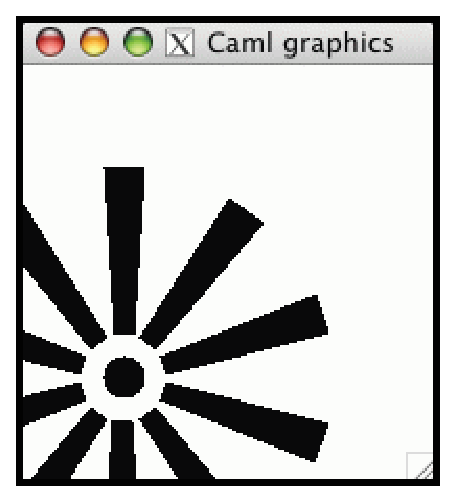
\includegraphics[scale=0.3]{graphics2}}

\section{Imperative objects}

\label{keyword:mutable(objects)}
\index{objects!imperative}
\index{mutable!object fields}
Next, it is natural to want to define a collection of items that acts like a single drawable object.
This time, let's define it imperatively, so that the collection includes a method \hbox{\lstinline/add/}
that adds an item to the collection by side-effect.  The syntax for a field that can be modified is
\hbox{\lstinline/val mutable $\nt{identifier}$ = $\nt{expression}$/}.

\label{keyword:<-(object-field-assignment)}
\index{<-!object field assignment}
\index{objects!mutable fields}
\begin{ocaml}
# let new_collection () =
object
   val mutable items = []
   method add item = items <- item :: items
   method draw = List.iter (fun item -> item#draw) items
   method transform matrix =
      {< items = List.map (fun item -> item#transform matrix) items >}
end;;
@
\begin{topoutput}
val new_collection :
  unit ->
  (< add : (< draw : unit; transform : 'c -> 'b; .. > as 'b) -> unit;
     draw : unit; transform : 'c -> 'a >
   as 'a) = <fun>
\end{topoutput}
@
\end{ocaml}
%
Apart from the inferred type, the definition is reasonably simple.  The field \hbox{\lstinline/items/} is
declared as mutable, and the method \hbox{\lstinline/add/} modifies it by side-effect (using \hbox{\lstinline/<-/}
for assignment).  Let's build a star.

\begin{ocaml}
let star =
   let poly = new_poly [|(0.0, 0.2); (0.1, 0.5); (0.0, 1.0); (-0.1, 0.5)|] in
   let star = new_collection () in
   star#add (new_circle (0.0, 0.0) 0.1);
   for i = 0 to 9 do
      let trans = transform#new_rotate (0.628 *. (float_of_int i)) in
      star#add (poly#transform trans)
   done;
   star;;
\end{ocaml}
%
Since the \hbox{\lstinline/star/} object is also a drawable object, we can also build a collection with
multiple stars.

\begin{ocaml}
let starry_night =
   let starry_night = new_collection () in
   let add_star (x, y, scale) =
      let trans = (transform#new_translate x y)
         ** (transform#new_scale scale scale) in
      starry_night#add (star#transform trans) in
   List.iter add_star
      [0.35, 0.50, 0.15;
       0.12, 0.95, 0.12;
       0.35, 0.95, 0.10;
       0.62, 0.90, 0.12;
       0.95, 0.85, 0.20];
   starry_night
\end{ocaml}
%
The images for the objects \hbox{\lstinline/star/} and \hbox{\lstinline/starry_night/} are shown below.

\begin{center}
\begin{tabular}{cc}
\hbox{\lstinline/star/} & \hbox{\lstinline/starry_night/}\\
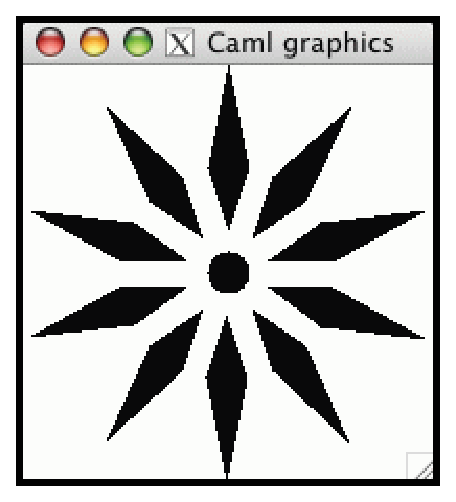
\includegraphics[scale=0.3]{graphics3}
&
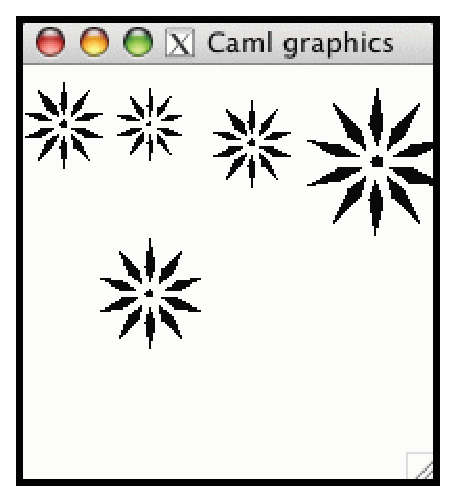
\includegraphics[scale=0.3]{graphics4}
\end{tabular}
\end{center}

\section{self: referring to the current object}

\label{objects:self}
\label{keyword:hash}
\index{self@\lstinline/self/}
\index{objects!self (the current object)}
Suppose we wish to define a method that is recursive, or a method that calls another method in the same
object.  In OCaml, the fields of an object can be referred to directly by name, but methods must
always use the syntax \hbox{\lstinline/$\nt{object}$#$\nt{method-name}$/}.  If we wish to call a method in
the current object, the object must first be named with the following syntax, where the name occurs in
parenthesis after the \hbox{\lstinline/object/} keyword.

\begin{ocaml}
object ($\nt{pattern}$) $\cdots$ end
\end{ocaml}
%
The pattern can use any identifier, but by convention the current object is usually
named \hbox{\lstinline/self/}.  It is often specified with a type as well.  The following form is conventional,
where the name \hbox{\lstinline/self/} refers to the current object, and \hbox{\lstinline/'self/} is its type.

\begin{ocaml}
object (self : 'self) $\cdots$ end
\end{ocaml}
%
Now that we have a name for the current object, let's define a collection method
\hbox{\lstinline/add_multiple n trans item/} that adds \hbox{\lstinline/n/} of the \hbox{\lstinline/item/}
to the collection, transforming each copy.  The easiest way to define the method is to make it
recursive.

\begin{ocaml}
let new_collection () =
   object (self : 'self)
      val mutable items = []
      method add item = items <- item :: items
      method add_multiple n matrix item =
         if n > 0 then begin
            self#add item;
            self#add_multiple (n - 1) matrix (item#transform matrix)
         end
      method draw = List.iter (fun item -> item#draw) items
      method transform matrix = $\cdots$
   end;;
\end{ocaml}
%
The expression \hbox{\lstinline/self#add item/} is a method call that adds the item to the current
collection, and \hbox{\lstinline/self#add_multiple/} is a recursive call.

\begin{center}
\begin{tabular}{cc}
\begin{minipage}[b]{3.5in}
\begin{ocamllisting}
let line =
   new_poly [|(0., 0.); (2., 0.); (2., 30.); (0., 30.)|];;
let xform =
   transform#new_translate 3. 0. ** transform#new_scale 1.1 1.1;;
let image = new_collection ();;
image#add_multiple 25 xform line;;
image#draw;;
\end{ocamllisting}
\end{minipage}
&
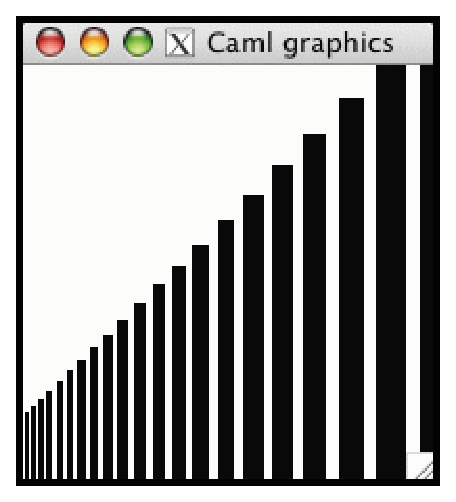
\includegraphics[scale=0.3]{graphics8}
\end{tabular}
\end{center}

\section{Initializers; private methods}

There is an important rule to keep in mind when constructing objects.

\begin{center}
---Field expressions may not refer to other fields, nor to \emph{self}.---
\end{center}
%
Here is an example.

\begin{ocaml}
# object
     val x = 1
     val x_plus_1 = x + 1
  end;;
@
\begin{topoutput}
Characters 38-39:
     val x_plus_1 = x + 1
                    ^
The instance variable x
cannot be accessed from the definition of another instance variable
\end{topoutput}
@
\end{ocaml}
%
The technical reason for this is that the object doesn't exist when the field values are being
computed, so it is an error to refer to the object or any of its fields and methods.

\label{keyword:initializer}
As one way of addressing this problem, objects can contain an \emph{initializer}, written
\hbox{\lstinline/initializer $\nt{expression}$/}.
The initializer expression is evaluated just after the object is created, but before it is used.  The
object exists at initialization, so it is legal to refer to its fields and methods in the
initializer.

\begin{ocaml}
# object
     val x = 1
     val mutable x_plus_1 = 0
     initializer
        x_plus_1 <- x + 1
  end;;
\end{ocaml}
%
Initializers are especially useful when an object has an invariant to be maintained, or when the
value of one field is derived from another.  For a more realistic example along these lines, let's
write a version of the polygon object that allows the polygon to be transformed in place (by
side-effect).

\begin{ocaml}
let new_imp_poly vertices =
   object
      val mutable vertices = vertices
      method draw = Graphics.fill_poly (Array.map int_coord vertices)
      method transform matrix = {< >}#transform_in_place matrix
      method transform_in_place matrix =
         vertices <- Array.map matrix#transform vertices
   end;;
\end{ocaml}
%
One potential source of inefficiency in this object is that the vertices are represented with floating-point coordinates, but must be drawn with integer coordinates.  The method \hbox{\lstinline/draw/} performs the conversion each time the object is drawn.

An alternative is to maintain two versions of the vertices, \hbox{\lstinline/float_vertices/}
and \hbox{\lstinline/int_vertices/}, with the invariant that
\hbox{\lstinline/int_vertices = Array.map int_coord float_vertices/}.
When one field is derived from another like this, it is usually best to define a method that handles
changes to the fields.  In this case, the method \hbox{\lstinline/set_vertices/} updates the object with
new coordinates.

\begin{ocaml}
# let new_imp_poly vertices =
object (self : 'self)
   val mutable float_vertices = [||]
   val mutable int_vertices = [||]
   method draw = Graphics.fill_poly int_vertices
   method transform matrix = {< >}#transform_in_place matrix
   method transform_in_place matrix =
      self#set_vertices (Array.map matrix#transform vertices)
   method private set_vertices vertices =
      float_vertices <- vertices;
      int_vertices <- Array.map int_coord float_vertices
   initializer
      self#set_vertices vertices
end;;
@
\begin{topoutput}
val new_imp_poly : (float * float) array ->
  < draw : unit;
    transform : (< transform : float * float -> float * float; .. > as 'a) -> unit;
    transform_in_place : 'a -> unit > = <fun>
\end{topoutput}
@
\end{ocaml}
%
The method \hbox{\lstinline/set_vertices/} is called in two places, 1) by the \hbox{\lstinline/initializer/} to set
the initial values of the vertices, and 2) by the method \hbox{\lstinline/transform_in_place/}, which
computes new values for the vertices.  The object reference \hbox{\lstinline/self/} is legal in the
initializer, allowing the method call \hbox{\lstinline/self#set_vertices/}.

\label{keyword:private}
This example also contains a \emph{private method}.  Private methods are defined with the syntax
\hbox{\lstinline/method private $\nt{identifier}$ = $\nt{expression}$/}.
They are used just like normal (public) methods, but they are not visible outside the object---they
don't even appear in the object type.

\section{Object types, coercions, and subtyping}

The types of the objects we have been creating are getting pretty complicated.
To make sense of it all, let's make some type definitions.  We don't really care about
giving the most general polymorphic types, so let's use exact non-polymorphic types instead.  We'll
call a drawable object a \hbox{\lstinline/blob/}.

\begin{ocaml}
type coord = float * float
type transform = < transform : coord -> coord >
type blob = < draw : unit; transform : transform -> blob >
type collection =
   < add : blob -> unit;
     draw : unit;
     transform : transform -> collection
   >
\end{ocaml}
%
Note that the type \hbox{\lstinline/collection/} differs from \hbox{\lstinline/blob/} in two ways.  A collection
has an extra method \hbox{\lstinline/add/}, and the method \hbox{\lstinline/transform/} returns another
collection, not a blob.

We can now annotate the object creation functions to get simpler types (the object definitions are
the same as before).

\begin{ocaml}
# let new_poly (vertices : coord array) : blob = object $\cdots$ end;;
@
\begin{topoutput}
val new_poly : coord array -> blob = <fun>
\end{topoutput}
@
# let new_circle (center : coord) radius : blob = object $\cdots$ end;;
@
\begin{topoutput}
val new_circle : coord -> float -> blob = <fun>
\end{topoutput}
@
# let new_collection () : collection = object $\cdots$ end;;
@
\begin{topoutput}
val new_collection : unit -> collection = <fun>
\end{topoutput}
@
\end{ocaml}
%
Now that the types are simplified, we run into a new issue: the actual object types do not match the
expected exact types.  For example, the method \hbox{\lstinline/transform/} now expects an object with
exactly one method (the method is also called \hbox{\lstinline/transform/}), but the real object has many more methods.
Here is what we get if we try to perform a transformation.

\begin{ocaml}
# let circle = new_circle (0.0, 0.0) 0.1;;
@
\begin{topoutput}
val circle : blob = <obj>
\end{topoutput}
@
# circle#transform (transform#new_translate 100.0 100.0);;
@
\begin{topoutput}
Characters 17-54:
  circle#transform (transform#new_translate 100.0 100.0);;
                   ^^^^^^^^^^^^^^^^^^^^^^^^^^^^^^^^^^^^^
This expression has type
  < multiply : ... > as 'a
but is here used with type transform
The second object type has no method multiply
\end{topoutput}
@
\end{ocaml}
%
The problem here is that the expression \hbox{\lstinline/(transform#new_translate 100.0 100.0)/} produces
an actual object with many methods, while the method \hbox{\lstinline/circle#transform/} expects an object
having exactly one method.  In principle, it should be fine to pass an object with more methods to
one that expects fewer---all the extra methods can simply be ignored.

\subsection{Coercions}

\label{keyword::>}
\index{objects!coercions}
\index{:>@\lstinline/:>/ object coercion}
In OCaml, such coercions are in fact legal, but they are not automatic.  This is in accord with the usual
OCaml policy that all coercions should be explicit; for example, integers are never coerced automatically
to floating-point values, the function \hbox{\lstinline/float_of_int/} must be written explicitly.

An explicit object coercion can be written two ways, as a ``single coercion'' or as a ``double coercion.''

\begin{center}
\begin{tabular}{ll}
    \lstinline/($\nt{object}$ :> $\nt{object-type}$)/ & single coercion\\
    \lstinline/($\nt{object}$ : $\nt{object-type}$ :> $\nt{object-type}$)/ & double coercion
\end{tabular}
\end{center}
%
The single coercion expression \hbox{\lstinline/($e$ :> $t$)/} coerces the object $e$ to have type $t$ (if
legal).  The double coercion expression \hbox{\lstinline/($e$ : $t_1$ :> $t_2$)/} means to consider first
that $e$ has type $t_1$, then coerce it to an object of type $t_2$.  In most cases, a single
coercion is sufficient.

\begin{ocaml}
# circle#transform (transform#new_translate 100.0 100.0 :> transform);;
@
\begin{topoutput}
- : blob = <obj>
\end{topoutput}
@
\end{ocaml}
%
For another example, consider the collection object, which contains a list of simple blobs.
If we want to add any other kind of object, it must be coerced.

\begin{ocaml}
# let image = new_collection ();;
@
\begin{topoutput}
val image : collection = <obj>
\end{topoutput}
@
# image#add (new_circle (0.0, 0.0) 0.1);;
@
\begin{topoutput}
- : unit = ()
\end{topoutput}
@
# image#add star;;
@
\begin{toperror}
Characters 10-14:
  image#add star;;
            ^^^^
This expression has type collection but is here used with type blob
The second object type has no method add
\end{toperror}
@
\end{ocaml}
%
That is as we expected, but the single coercion doesn't work either.

\begin{ocaml}
# image#add (star :> blob);;
@
\begin{topoutput}
Characters 11-15:
  image#add (star :> blob);;
             ^^^^
This expression cannot be coerced to type
  blob = < draw : unit; transform : transform -> blob >;
...
This simple coercion was not fully general. Consider using a double coercion.
\end{topoutput}
@
\end{ocaml}
%
The real error message is quite long, most of it has been elided.  The last line suggests using a
double coercion, so we try that.  Finally, success.

\begin{ocaml}
# star;;
@
\begin{topoutput}
- : collection = <obj>
\end{topoutput}
@
# image#add (star : collection :> blob);;
@
\begin{topoutput}
- : unit = ()
\end{topoutput}
@
\end{ocaml}
%
\index{coercions (single \emph{vs}.{} double)}
%
Why does the single coercion sometimes work, but at other times the double coercion is required?
The complete technical explanation is complicated and has to do with the specific algorithm used for
type inference.  The simplest rule is this: if the compiler complains about a single coercion, try
replacing it with a double coercion.  If you would like to know the real reason, a bit of
explanation might be helpful.

Internally, the compiler uses only double coercions.  Whenever the compiler encounters a single
coercion \hbox{\lstinline/($e$ :> $t_2$)/} it constructs a double coercion
%
\hbox{\lstinline/($e$ : $t_1$ :> $t_2$)/} by inferring the \emph{most general expected type} $t_1$.
However, this fails if there is no unique most general expected type.  The general guidelines can be
stated as follows.
%
\begin{quote}
A single coercion \hbox{\lstinline/($e$ :> $t_2$)/} may fail if:
\begin{itemize}
\item the type $t_2$ is recursive, or
\item the type $t_2$ has polymorphic structure.
\end{itemize}
If either condition holds, use a double coercion \hbox{\lstinline/($e$ : $t_1$ :> $t_2$)/}.
\end{quote}
%
In our example, the single coercion \lstinline/(transform#new_translate 100.0 100.0 :> transform)/
is successful because the type \hbox{\lstinline/transform/} is neither recursive nor polymorphic.  However,
the coercion \hbox{\lstinline/(star :> blob)/} fails because the type \hbox{\lstinline/blob/} is recursive.  The
compiler doesn't consider the actual type of the expression, so even though we know
\hbox{\lstinline/star/} has type \hbox{\lstinline/collection/}, it is still necessary to write the double coercion
\hbox{\lstinline/(star : collection :> blob)/}.  

\labelsubsection{subtyping}{Subtyping}

\index{objects!subtyping}
\index{subtyping!relation}
\index{<:@$\subtype$ relation}
That's not the entire story of course, because not all coercions \hbox{\lstinline/($e$ : $t_1$ :> $t_2$)/}
are legal.  There are two necessary conditions: first, expression $e$ should have type $t_1$; and
second, type $t_1$ must be a subtype of $t_2$.

We say that a type $t_1$ is a \emph{subtype} of $t_2$, written $t_1 \subtype t_2$, if values of type
$t_1$ can be used where values of type $t_2$ are expected.  It may be confusing that the
symbols \hbox{\lstinline$:>$} (the coercion operator) and $\subtype$ (the
subtyping relation) look like they point in opposite directions.  It may be
helpful to remember that the former is an operator, and the latter is
a relation not belonging to the syntax of the language.

Consider the following type definitions: an \hbox{\lstinline/animal/} eats, and a \hbox{\lstinline/dog/} also
barks.

\begin{ocaml}
type animal = < eat : unit >
type dog = < eat : unit; bark : unit >
\end{ocaml}
%
The subtyping relation $\mt{dog} \subtype \mt{animal}$ holds because a \hbox{\lstinline$dog$} object
has all the methods that an animal has with the same type, and so a dog object $e$ can be used wherever
an \hbox{\lstinline$animal$} object is expected (so the coercion \hbox{\lstinline/($e$ : dog :> animal)/} is legal).

\subsubsection{Width and depth subtyping}
\label{section:width-subtyping}

\index{subtyping!width}
\index{subtyping!depth}
Subtyping for object types takes two forms, called \emph{width} and \emph{depth} subtyping.  Width
subtyping means that an object type $t_1$ is a subtype of object type $t_2$ if $t_1$ implements all
the methods (and possibly more) of $t_2$ with the same method types.  The order of methods in an
object type doesn't matter, so we can write this as follows, where we use the
notation \hbox{\lstinline/$f_{1..n}$ : $t_{1..n}$/} to represent $n$ method
declarations \hbox{\lstinline/$f_i$ : $t_i$/} for $i \in \{ 1, 2, \ldots, n \}$.

\begin{ocaml}
< $f_{1..n}$ : $t_{1..n}$, $g_{1..m}$ : $s_{1..m}$ > $\subtype$ < $f_{1..n}$ : $t_{1..n}$ >
\end{ocaml}
%
The subtyping relation $\mt{dog} \subtype \mt{animal}$ follows from width subtyping, because class
type \hbox{\lstinline$dog$} implements the \hbox{\lstinline$eat$} method, the only method in
the \hbox{\lstinline$animal$} class type.

\begin{ocaml}
< eat : unit; bark : unit > $\subtype$ < eat : unit >
\end{ocaml}
%
Depth subtyping means that an object type $t_1$ is a subtype of
$t_2$ if the two types have the same methods, but the method
types in $t_1$ are subtypes of the corresponding types in
$t_2$.  This rule is usually written as follows, as an \emph{inference
rule}, where the subtyping properties above the horizontal line imply
the subtyping property below the line.  We read it informally as
follows, ``If each method type $s_i$ is a subtype of method type
$t_i$, then the object type \hbox{\lstinline/< $f_{1..n}$ : $s_{1..n}$ >/}
is a subtype of the object type \hbox{\lstinline/< $f_{1..n}$ : $t_{1..n}$ >/}.''

\begin{center}
\begin{tabular}{c}
$s_i \subtype t_i$ \quad (for each $i \in \{ 1, \ldots, n \}$)\\
\hline
\hbox{\lstinline/< $f_{1..n}$ : $s_{1..n}$ > $\subtype$ < $f_{1..n}$ : $t_{1..n}$ >/}
\end{tabular}
\end{center}
%
\index{covariant types}
\index{contravariant types}
\index{invariant types}
In general, the method types may include various type constructors for
tuples, lists, records, functions, other objects, \emph{etc}.  Each type
constructor in OCaml has its own subtyping rules describing how the
type construction varies in terms of its component types.  These
variances can be \emph{covariant}, meaning that the construction
varies in the same way as a component type; \emph{contravariant},
meaning the construction varies oppositely to a component type;
or \emph{invariant}, which means that it is neither purely covariant
nor purely contravariant.

For example, consider the tuple type \hbox{\lstinline/$t_1$ * $t_2$/}, which
is covariant in both types $t_1$ and $t_2$.  If we have two dogs
\hbox{\lstinline$dog * dog$}, then we also have two animals
\hbox{\lstinline$animal * animal$} (so 
\hbox{\lstinline/dog * dog $\subtype$ animal * animal/}).
The inference rule for pairs is specified as follows.

$$\infer{(s_1 * s_2) \subtype (t_1 * t_2)}{s_1 \subtype t_1 & s_2 \subtype s_2}$$

\subsubsection{Function subtyping}

\index{subtyping!function types}
Nearly all type constructors in OCaml are covariant over all their
component types, but there are two exceptions.  One is that types that specify
mutable values are always invariant.  The other exception is more
interesting, for the function type.  A function
type \hbox{\lstinline/$t_1$ -> $t_2$/} is covariant in its range type
$t_2$, but \emph{contravariant} in the domain type $t_1$.  This
property is written as follows.

$$\infer{(s_1 \mathrel{\mt{->}} s_2) \subtype (t_1 \mathrel{\mt{->}} t_2)}
{t_1 \subtype s_1 & s_2 \subtype t_2}$$
%
The contravariance in function types is the source of many problems in
the design of object-oriented programming languages, and it can be
difficult to understand.  To get some intuition, consider a
function \hbox{\lstinline$feed$} for feeding an animal.

\begin{ocaml}
# let feed (x : animal) = x#eat;;
@
\begin{topoutput}
val feed : animal -> unit = <fun>
\end{topoutput}
@
\end{ocaml}
%
When calling the function, we can pass it an \hbox{\lstinline$animal$} object
or a \hbox{\lstinline$dog$} object---both support the \hbox{\lstinline$eat$}
method.  Thus, if we like, we can coerce the function to have type
\hbox{\lstinline$dog -> unit$}.

\begin{ocaml}
# let feed_dog = (feed : animal -> unit :> dog -> unit);;
@
\begin{topoutput}
val feed_dog : dog -> unit = <fun>
\end{topoutput}
@
\end{ocaml}
%
Now consider an barking function for dogs.

\begin{ocaml}
# let do_bark (x : dog) = x#bark;;
@
\begin{topoutput}
val do_bark : dog -> unit = <fun>
\end{topoutput}
@
\end{ocaml}
%
We can't pass a plain \hbox{\lstinline$animal$} object
to \hbox{\lstinline$do_bark$}, because animals do not bark in general.  In
general, we \emph{cannot} use a function of type
\hbox{\lstinline$dog -> unit$} in places where a function of type
\hbox{\lstinline$animal -> unit$} is
expected.

\begin{ocaml}
# (do_bark : dog -> unit :> animal -> unit);;
@
\begin{toperror}
Characters 0-41:
  (do_bark : dog -> unit :> animal -> unit);;
  ^^^^^^^^^^^^^^^^^^^^^^^^^^^^^^^^^^^^^^^^^
Type dog -> unit is not a subtype of type animal -> unit 
Type animal = < eat : unit > is not a subtype of type
  dog = < bark : unit; eat : unit > 
\end{toperror}
@
\end{ocaml}

\subsubsection{Subtyping of recursive object types}

Finally, let's consider subtyping for recursive object types.  In this case, the subtyping rule is circular: first, assume that the subtyping relationship holds, then prove that it holds.  Don't worry---in this particular case the circular argument is sound.

For example, consider the argument that a \hbox{\lstinline/collection/} is a \hbox{\lstinline/blob/}.  The types
are recursive, so we first assume that the relation holds, and then prove it.  Here is the argument.

\begin{itemize}
\item Assume: \hbox{\lstinline/collection $\subtype$ blob/}.
\item Show:

\begin{tabular}{ccc}
\begin{minipage}{2in}
\begin{ocamllisting}
< add : blob -> unit;
  draw : unit;
  transform : transform -> collection
>
\end{ocamllisting}
\end{minipage}
&
$\subtype$
&
\begin{minipage}{2in}
\begin{ocamllisting}
< draw : unit;
  transform : transform -> blob
>
\end{ocamllisting}
\end{minipage}
\end{tabular}

\item From width subtyping, we can ignore the \hbox{\lstinline/add/} method.

\begin{tabular}{ccc}
\begin{minipage}{2in}
\begin{ocamllisting}
< draw : unit;
  transform : transform -> collection
>
\end{ocamllisting}
\end{minipage}
&
$\subtype$
&
\begin{minipage}{2in}
\begin{ocamllisting}
< draw : unit;
  transform : transform -> blob
>
\end{ocamllisting}
\end{minipage}
\end{tabular}

\item The \hbox{\lstinline/draw/} methods have the same type.
The \hbox{\lstinline/transform/} method is justified by depth subtyping.
We must show the following.

\begin{ocaml}
transform -> collection $\subtype$ transform -> blob
\end{ocaml}

\item Functions are covariant in the range type.  The final goal is the following.

\begin{ocaml}
collection $\subtype$ blob
\end{ocaml}

This follows by assumption.
\end{itemize}

\section{Narrowing}
\label{section:narrowing}

\index{subtyping!narrowing}
\index{narrowing}
In object-oriented programming, \emph{narrowing} is the ability to coerce an object to one of its
subtypes---the opposite of a normal coercion.  This is commonly used when the actual type of an
object has been lost due to a coercion somewhere else in the program.  For example, suppose we have
defined some types for cats and dogs.  If we want a list that contains both cats and dogs, the
elements of the list must coerced to a common type, in this case the supertype \hbox{\lstinline/animal/}.

\begin{ocaml}
type animal = < eat : unit >
type dog = < eat : unit; bark : unit >
type cat = < eat : unit; meow : unit >

let fido : dog = $\cdots$
let daphne : cat = $\cdots$

let animals = [(fido :> animal); (daphne :> animal)]
\end{ocaml}
%
Because of the coercion, the methods \hbox{\lstinline/bark/} and \hbox{\lstinline/meow/} have been lost, which can
be a potential problem.  Languages that support narrowing usually include a ``typecase'' to perform
a case analysis on an object's actual type.  The following function illustrates how a typecase
would be written, presented in OCaml-style pseudo-code.

\begin{ocaml}
(* THIS IS NOT LEGAL OCAML CODE *)
let chorus (animals : animal list) =
   List.iter (fun animal ->
      if @\textit{animal instanceof dog}@ then (animal :> dog)#bark
      else if @\textit{animal instanceof cat}@ then (animal :> cat)#meow) animals
\end{ocaml}
%
Narrowing is \textbf{not permitted} in OCaml.  Period.  First, we'll give some arguments why
narrowing is undesirable, then we'll describe how to do it anyway.

\subsection{Why narrowing is bad}

The usual argument against narrowing is that it is unsound.  Actually, it is probably more accurate
to say that it isn't known whether there is a useful, general form of narrowing that is compatible
with the OCaml type system.

We might leave it at that, but there are good \emph{design} principles that also argue against
narrowing.  One of the principal benefits of object-oriented programming is that the responsibility
of implementation is shifted to the object, away from the client.  The need for case analysis is
reduced because of dynamic lookup, which ensures that the code that is executed is always appropriate
to the object.

Looking at our example, the problem is that a single concept, let's call it ``\hbox{\lstinline/speak/},'' is named in two
different ways, \hbox{\lstinline/bark/} and \hbox{\lstinline/meow/}.  A better implementation would use the same
name in both cases, perhaps also keeping the species-specific name.

\begin{ocaml}
type animal = < eat : unit; speak : unit >
type dog = < eat : unit; speak : unit; bark : unit >
type cat = < eat : unit; speak : unit; meow : unit >
type lizard = < eat : unit; speak : unit; sleep : unit >
let fido : dog = object (self) method speak = self#bark $\cdots$ end
let daphne : cat = object (self) method speak = self#meow $\cdots$ end
let fred : lizard = object (self) method speak = () $\cdots$ end
let animals = [(fido :> animal); (daphne :> animal); (fred :> animal)]

let chorus (animals : animal list) =
   List.iter (fun animal -> animal#speak) animals
\end{ocaml}
%
No case analysis is necessary; it is the responsibility of each animal to decide how it will speak.

In other cases, the abstraction must be changed to avoid the lossy coercion.  For example, one might
decide that, out of a collection of animals, the dogs should bark but all other animals should
remain silent.  The solution in that case is to avoid the coercion in the first place.  If it is
important to know which of the animals are dogs and which are cats, then a single list of animals is
not appropriate.  Multiple lists should be used instead.

\subsection{Implementing narrowing}

If, despite these arguments, you still wish to use narrowing, it is fairly easy to implement.
There are two things we need: a runtime ``tag'' that indicates what the actual type of an object is,
and a ``typecase'' for case analysis over the tag.  The tags should be \emph{open} so that new
subclasses can be added, which leaves us with two choices: polymorphic variants
(Section~\ref{section:open-union-types}), or exceptions.  We'll use exceptions for illustration
because the types are easier to write down.  The main idea is to define a method \hbox{\lstinline/actual/}
that returns the actual object.

\label{page:narrowing-with-exceptions}
\begin{ocaml}
type narrowable_object = < actual : exn >
type animal = < actual : exn; eat : unit >
type dog = < actual : exn; eat : unit; bark : unit >
type cat = < actual : exn; eat : unit; meow : unit >
exception Dog of dog
exception Cat of cat

let fido : dog = object (self) method actual = Dog self $\cdots$ end
let daphne : cat = object (self) method actual = Cat self $\cdots$ end

let animals = [(fido :> animal); (daphne :> animal)]

let chorus (animals : animal list) =
   List.iter (fun animal ->
      match animal#actual with
         Dog dog -> dog#bark
       | Cat cat -> cat#meow
       | _ -> ()) animals
\end{ocaml}
%
The idea here is to define a constructor for each actual type of object (defined here as the
exceptions \hbox{\lstinline/Dog/} and \hbox{\lstinline/Cat/}).  The method \hbox{\lstinline/actual/} returns a tagged
object, and the case analysis uses a \hbox{\lstinline/match/} expression.  The use of exceptions is a
technicality; Exercise~\ref{exercise:narrowing-with-polymorphic-variants} discusses narrowing using
polymorphic variants.

\section{Alternatives to objects}

The objects we have seen in this chapter are simple, serving mainly to encapsulate some data
together with functions that operate on that data.  In many ways, they are similar to abstract data
types.  In fact, much of what we have done in this chapter can also be done using the module
system.  However, there are two key differences: 1) with objects, the type of the data is entirely hidden,
and 2) objects are first-class values, while modules are not.  For example, a module to implement
a polygon might be written as follows.

\begin{ocaml}
module type PolySig = sig
   type poly
   val create : (float * float) array -> poly
   val draw : poly -> unit
   val transform : poly -> transform -> poly
end;;

module Poly : PolySig =
   type t = (float * float) array
   let create vertices = vertices
   let draw vertices = Graphics.fill_poly (Array.map int_coord vertices)
   let transform matrix = Array.map matrix#transform vertices
end;;
\end{ocaml}
%
The main problem with this approach is that, even though the data
type \hbox{\lstinline/Poly.poly/} is abstract, it is explicit.  A polygon has
type \hbox{\lstinline/Poly.poly/}; a circle would have a similar type
like \hbox{\lstinline/Circle.circle/}, \emph{etc}.  This means, for example, that one cannot create a list
containing both polygons and circles without further effort.

In Exercise~\ref{exercise:record-objects1}, we suggested that a simplified object could be
represented as a record of methods.  In fact, this is quite similar to what we have seen in this
chapter, except for functional update.  Note the recursive call to the function \hbox{\lstinline/new_poly/}
in the following implementation.

\begin{ocaml}
type blob =
   { draw : unit -> unit;
     transform : transform -> blob
   }

let rec new_poly vertices =
   { draw = Graphics.fill_poly (Array.map int_coord vertices);
     transform = (fun matrix -> new_poly (Array.map matrix#transform vertices))
   }
\end{ocaml}
%
We can build many object features from records and other parts of the language, but the fact
is that the simple objects we have seen in this chapter provide a simple, useful programming model.
However, we are still missing one of the most important features, \emph{inheritance}, the topic of
the next chapter.

% -*-
% Local Variables:
% Mode: LaTeX
% fill-column: 100
% TeX-master: "paper"
% TeX-command-default: "LaTeX/dvips Interactive"
% End:
% -*-
% vim:tw=100:fo=tcq:
